% 
% Licensed to the Apache Software Foundation (ASF) under one
% or more contributor license agreements.  See the NOTICE file
% distributed with this work for additional information
% regarding copyright ownership.  The ASF licenses this file
% to you under the Apache License, Version 2.0 (the
% "License"); you may not use this file except in compliance
% with the License.  You may obtain a copy of the License at
% 
%   http://www.apache.org/licenses/LICENSE-2.0
% 
% Unless required by applicable law or agreed to in writing,
% software distributed under the License is distributed on an
% "AS IS" BASIS, WITHOUT WARRANTIES OR CONDITIONS OF ANY
% KIND, either express or implied.  See the License for the
% specific language governing permissions and limitations
% under the License.
% 

    \section{Jobs Page}
    \label{sec:ws.jobs-page}
        The Web Server's home page is also the Jobs page. This page has links to all the rest of the content 
        at the site and shows the status of all the jobs in the system. 
    
        The Jobs page contains the following columns: 

        \begin{description}

            \item[Id] \hfill \\
              This is the ID as assigned by {\DUCC}. This field is hyperlinked to a
              \hyperref[sec:ws-job-details]{Job Details} page for that job that shows the breakdown of
              all the processes assigned to the job and their state.
              
            \item[Start] \hfill \\
              This is the time the Job is accepted into {\DUCC}.
              
            \item[Duration] \hfill \\
              This shows two times.  In green the length of time the job has been running.  In black is
              the estimated time of completion, based on current resources and remaining work.  When
              the job completes, the time shown is the total elapsed time of the job.
                            
            \item[User] \hfill \\
              This is the userid of the job owner.
              
            \item[Class] \hfill \\
              This is the resource class the job is submitted to.
              
            \item[State] \hfill \\
              This shows the state of the job.  The normal job progression is shown below, with an
              explanation of what each state means.
              \begin{description}
                  \item[Received] - The job has been vetted, persisted, and assigned a unique ID. 
                  \item[WaitingForDriver] - The job is waiting for the Job Driver to initialize. 
                  \item[WaitingForServices] - The job is waiting for verification from the
                    Service Manager that required services are started and responding.  This may
                    cause {\DUCC} to start services if necessary.  In that even this state will
                    persist until all pre-requisite services are ready.
                  \item[WaitingForResources] - The job is waiting to be scheduled. In busy
                    systems this may require preemption of existing work.  In that case this
                    state will persist until preemption is complete.
                  \item[Initializing] - The job initializing. Usually this
                    is the UIMA-AS initialization phase.  In the default configuration, only
                    two (2) processes are allocated by the Resource Manager.  No additional
                    resources are allocated until at least one of the new processes successfully
                    completes initialization.  Once initialization is complete the Resource Manager
                    will double the number of allocated processes until the user's fair share of
                    the resources is attained.
                  \item[Running] - At least one process is now initialized and running. 
                  \item[Completing] - The last work item has completed and {\DUCC} is freeing resources.
                    If the job had many resources allocated at the time the job exited this state
                    will persist until all allocated resources are freed.
                  \item[Completed] - The job is complete. 
              \end{description}
                  
            \item[Reason or Extraordinary Status] \hfill \\

              % See this structure:
              % org.apache.uima.ducc.transport.event.common.IDuccCompletionType
              
              This field contains miscellaneous information pertaining to the job.  If the job exits
              the system for any reason, that reason is shown here.  If the job's pre-requisite
              services are unavailable (or ailing) that fact is displayed here.  If there is a
              job monitor running, that fact is shown here.  Most of the values for this field
              support ``hovers'' containing additional information about the reason.
         
              \begin{description}
                  \item[EndOfJob] - The job and completed ran with no errors. 
                  \item[Error] - All work items are processes but at least one had an error. 
                  \item[CanceledByDriver] - The Job Driver (JD) terminated the job. The reason for
                    termination is seen by hovering over the text with your mouse.
                  \item[CanceledBySystem] - The job was canceled because {\DUCC} was shutdown. 
                  \item[CanceledBySser] - The job owner or {\DUCC} administrator canceled the job. 
                  \item[Cancel Pending] - The job has been canceled and is not yet fully evicted
                    from the system.
                  \item[DriverInitializationFailure] - The Job Driver (JD) process is unable to initialize. Hover over 
                    the field with your mouse for details (if any are available), and check your JD log. 
                  \item[DriverProcessFailed] - The Job Driver (JD) process failed for some reason. Hover over the 
                    field with your mouse for details (if any), and check your JD log. 
                  \item[MonitorActive] The job has a console monitor active.  This is enabled with the
                    job's ``wait\_for\_completion'' parameter on job submission.
                  \item[ServicesUnavailable] - The job declared a dependency on one or more services, and the 
                    Service Manager (SM) cannot find or start the required service. 
                  \item[Premature] - The job was terminated for some unknown reason before all work items were 
                    processed. Check the JP logs for details. 
                  \item[ProcessInitializationFailure] - Too many processes failed during
                    initialization and the job was canceled by {\DUCC}.  Check the JP logs for the
                    reason.
                  \item[ProcessFailure] - Too many processes failed while running and {\DUCC} canceled
                    the job.  Check the JP logs for the reason.
                  \item[ResourcesUnavailable] - The Resource Manager (RM) is unable to allocate resources for 
                    the job. For non-preemptable jobs this could be because the limit on that type of allocation is 
                    reached, or all the hosts are already allocated and work cannot be preempted to make space for 
                    it. For all jobs, it could be because the job class is invalid. 
                    \item[{\em service\_name}] If there is a service name in this field it indicates the job is
                      dependent on the service but the service is not responding to the {\DUCC} Service Monitor's
                      pinger.
              \end{description}

            \item[Services] \hfill \\
              This is the number of services the job has declared dependencies on.  There is a ``hover'' that
              shows the ids of the services, if any.

            \item[Processes] \hfill \\
              This is the number of processes currently assigned to the job.

            \item[Init Fails] \hfill \\
              This is the total number of initialization failures experienced by the job. This
              field is hyperlinked to pages with log excerpts highlighting the specific failures.
              
            \item[Run Fails] \hfill \\
              This is the total number of process failures experienced by the job. This field is
              hyperlinked to pages with log excerpts highlighting the specific failures.
              
            \item[PgIn] This is the number of page-in events, over all processes, on the machines
              running the job.

            \item[Swap] This is the total swap space, over all the processes, being used by the job.

            \item[Memory] \hfill \\
              This is the declared memory size of the job
              
            \item[Total] \hfill \\
              This is the total number of work items declared by the job.
              
            \item[Done] \hfill \\
              This is the total number of work items successfully completed for the job.
              
            \item[Error] \hfill \\
              This is the total number of exceptions thrown or other errors experienced by work
              items. This field is hyperlinked to pages containing log excerpts highlighting
              the failures.
              
            \item[Dispatch] \hfill \\
              This is the total number CASs that are currently dispatched. 

              This usually represents the quantity derived from the following formula:
\begin{verbatim}              
     min( (initialized.processes * threads.per.process), (incomplete.work.items - errors) )
\end{verbatim}

              The actual number is a measured number, not a calculated number, and may differ
              slightly from the formula if the measurement is taken immediately after process
              start-up, or in the time between a work item completing and a new one being
              dispatched.
              
            \item[Retry] \hfill \\
              This is the number of CASs that were retried for any reason.  Reasons for retry
              include preemption for fair-share, work-item timeout, or error conditions.

              Note: If a work item in any process fails, the entire process is considered
              suspect, and all work-items in the process are terminated.  Work items in the
              process which did not have errors are re-dispatched (retried) to a different
              process.
              
            \item[Preempt] \hfill \\
              This is the total number of processes that have been preempted to make room for
              other work due to Fair Share.
              
            \item[Description] \hfill \\
              This is the description string from the $--$description string from submit.
            \end{description}

    \begin{figure}[ht!]
    \centering
    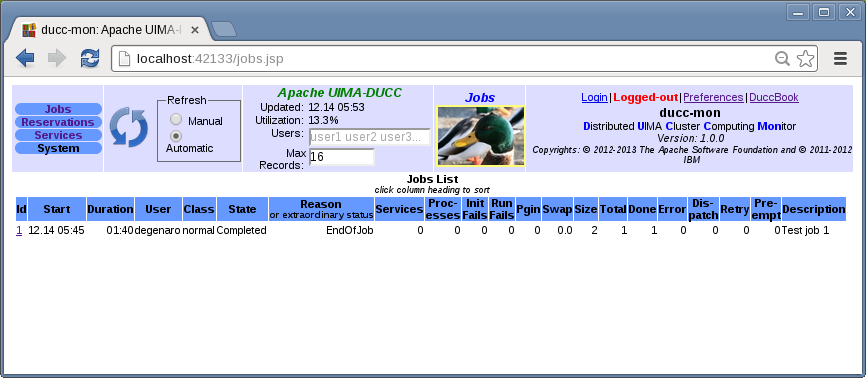
\includegraphics[width=90mm]{images/ducc-webserver/Jobs.png}
    \caption{Jobs Page}
    \end{figure}
            
